% This is based on "sig-alternate.tex" V1.9 April 2009
% This file should be compiled with V2.4 of "sig-alternate.cls" April 2009
%
\documentclass{report}

\usepackage[english]{babel}
\usepackage{graphicx}
\usepackage{tabularx}
\usepackage{subfigure}
\usepackage{enumitem}
\usepackage{url}


\usepackage{color}
\definecolor{orange}{rgb}{1,0.5,0}
\definecolor{lightgray}{rgb}{.9,.9,.9}
\definecolor{java_keyword}{rgb}{0.37, 0.08, 0.25}
\definecolor{java_string}{rgb}{0.06, 0.10, 0.98}
\definecolor{java_comment}{rgb}{0.12, 0.38, 0.18}
\definecolor{java_doc}{rgb}{0.25,0.35,0.75}

% code listings

\usepackage{listings}
\lstloadlanguages{Java}
\lstset{
	language=Java,
	basicstyle=\scriptsize\ttfamily,
	backgroundcolor=\color{lightgray},
	keywordstyle=\color{java_keyword}\bfseries,
	stringstyle=\color{java_string},
	commentstyle=\color{java_comment},
	morecomment=[s][\color{java_doc}]{/**}{*/},
	tabsize=2,
	showtabs=false,
	extendedchars=true,
	showstringspaces=false,
	showspaces=false,
	breaklines=true,
	numbers=left,
	numberstyle=\tiny,
	numbersep=6pt,
	xleftmargin=3pt,
	xrightmargin=3pt,
	framexleftmargin=3pt,
	framexrightmargin=3pt,
	captionpos=b
}

% Disable single lines at the start of a paragraph (Schusterjungen)

\clubpenalty = 10000

% Disable single lines at the end of a paragraph (Hurenkinder)

\widowpenalty = 10000
\displaywidowpenalty = 10000
 
% allows for colored, easy-to-find todos

\newcommand{\todo}[1]{\textsf{\textbf{\textcolor{orange}{[[#1]]}}}}

% consistent references: use these instead of \label and \ref

\newcommand{\lsec}[1]{\label{sec:#1}}
\newcommand{\lssec}[1]{\label{ssec:#1}}
\newcommand{\lfig}[1]{\label{fig:#1}}
\newcommand{\ltab}[1]{\label{tab:#1}}
\newcommand{\rsec}[1]{Section~\ref{sec:#1}}
\newcommand{\rssec}[1]{Section~\ref{ssec:#1}}
\newcommand{\rfig}[1]{Figure~\ref{fig:#1}}
\newcommand{\rtab}[1]{Table~\ref{tab:#1}}
\newcommand{\rlst}[1]{Listing~\ref{#1}}

% General information

\title{Ripple - The future of local social networking\\
\normalsize{Distributed Systems -- Project Proposal}}
\subtitle{subtitle}

% Use the \alignauthor commands to handle the names
% and affiliations for an 'aesthetic maximum' of six authors.

\numberofauthors{1} %  in this sample file, there are a *total*
% of EIGHT authors. SIX appear on the 'first-page' (for formatting
% reasons) and the remaining two appear in the \additionalauthors section.
%
\author{
% You can go ahead and credit any number of authors here,
% e.g. one 'row of three' or two rows (consisting of one row of three
% and a second row of one, two or three).
%
% The command \alignauthor (no curly braces needed) should
% precede each author name, affiliation/snail-mail address and
% e-mail address. Additionally, tag each line of
% affiliation/address with \affaddr, and tag the
% e-mail address with \email.
%
% 1st. author
\alignauthor \normalsize{Carl Friess, Isaak Hanimann, Sven Knobloch, Laurin Paech,  Sebastian Winberg, David Yenicelik}\\
	\affaddr{\normalsize{cfriess  15-943-111, isaakh 15-913-312, knsven 14-945-166, lpaech 15-944-242, winbergs 15-941-222,  yedavid 15-944-366}}\\
	\email{\normalsize{cfriess@student.ethz.ch, isaakh@student.ethz.ch, knsven@student.ethz.ch, lpaech@student.ethz.ch, winbergs@student.ethz.ch, yedavid@student.ethz.ch}}
}


\begin{document}

\maketitle

\begin{abstract}
We propose a novel social networking application for sharing photos in close physical proximity. 
A user can take a picture, which is then broadcasted to all phones that are part of the network and in the direct vicinity. \\
To increase speed and reduce operating costs, the Android application does not solely rely on high-bandwidth connections with a centralized server, but rather uses a distributed peer to peer network to transmit photos between individual nodes.
Our proposed app utilizes a combination of the Bluetooth Low Energy and BitTorrent protocols, as well as a custom RESTful HTTP API.\\
The fundamental transfer of image files is done using BitTorrent. A central tracker will facilitate the discovery of nodes in accordance with the BitTorrent protocol. A receiving node will then download the image form the initial node and from other nodes, which have already completed the download. The tracker will use a JavaScript BitTorrent implementation \todo{Link} executed in a node.js environment hosted on a AWS EC2 instance.\\
Devices use the Bluetooth Low Energy Protocol for close proximity device discovery and for transmitting identifying information of  the broadcasted images.\\
A centralized server further allows devices to retrieve torrent files, which are necessary for the BitTorrent protocol.\\
Our goal is to have a fully-working prototype with the proposed architecture, where a single node delivers to another node, and where a node can ping other nodes if it is 'missing' a photo.  \todo{???}
All participating, delivering and receiving nodes are determined by the tracker.
\end{abstract}

\section{Introduction}

We first introduce a few definitions.

\begin{enumerate}
\item \textbf{ripple} \textit{(noun)}: A photo that is being shared with anyone nearby from a central person's smartphone. We will use the words 'ripple' and 'photo' interchangeably. 
\item \textbf{to ripple} \textit{(verb)}: When person A shares a photo (the ripple), and person B decides to share it again, the photo has 'rippled' once as it propagated over one person since the initial share.
\item \textbf{tracker}: A central server handling the distribution logic
\item \textbf{AWS}: Amazon Web Services. The cloud, which will act as the tracker.
\item \textbf{P2P}: Peer to peer
\item \textbf{$ n $}: The number of nodes in observed network. In our case, these nodes will be android devices.
\end{enumerate}

\subsection{Problem statement}
There have been numerous social networking applications that connect people over a range of topics. 
Such services include Instagram and Snapchat, where a person shares his or her moments with a local group of people, namely their friends. 
However, none of these services share their appreciated moments with people nearby (measured by geographical proximity). 
As such, we propose Ripple: a local social networking app where people share their appreciated moments with anyone near them.

\subsection{Application scenario}
We propose a novel Android application and demostrate it's application scenario by first defining a group of people, namely \textit{Alice}, \textit{Bob}, \textit{Charlie}, \textit{Daniel}.
Alice sees a human rights demonstration, and captures a symbolic and emotionally photo of a police officer shouting at a demonstrator. 
Bob, who is home but nearby the demonstrations  receives this photo and deeply appreciates this moment. 
He decides to share this photo again. Due to the rules of our network, this picture is shared with anyone close to Bob. Because Charlie and Daniel also have the Ripple app installed, and are physically close enough to Bob, Charlie and Daniel also receive this photo. They again have the opportunity to further share this photo, or simply 'drop' it and block further 'propagation' of this photo.

\subsection{Motivation}
The idea behind the above described mechanism is that the mass forms a selective filter over what content to share. 
If a ripple is 'good', it has the chance to be propagated over all ripple users, as the photo will be propagated repeatedly. 
This allows the entire userbase to experience pictures that are meaningful to the user, for the reason that the receiver is 'in proximity' to the event. 
More specifically, if the first share indicates appreciation of the picture, and each additional share indicates consistence in this appreciation, then - by induction - everyone feels appreciation of this picture.
Generally, the more important the event is, the more 'close' a person feels to this to this event. 
If, however, a photo is of bad quality or is not appreciated, local users will quickly stop the photo to be propagated, forming a natural blockade for any non-appreciated pictures.

\subsection{Challenges}
This task proposes a challenge because 

\begin{enumerate}
\item We work with a theoretically exponentially increasing number of users receiving a single ripple causing possibly high loads if deployed on a centralized server.
Any high-loaded point in the delivery-network could form a point of failure.
\item We must find a dynamic way for users to receive enough ripples to be engaged, but at the same time not to be spammed with photos.
\end{enumerate}

\section{System Overview}


\subsection{System Architecture}
We describe the distributed system architecture with regards to the above presented challenges. \\

We intend to solve 1.) by a \textit{P2P} (peer to peer) network which makes a central server redundant.
Instead of downloading all photos from a central server, each phone is a node and independently transmits it's captured image directly to it's close neighbours. 
It also has the benefit that we remove any single point of failure within the system, as there are multiple possible paths to a receiver from a sender in the network of phone-nodes (assuming multiple people are in physical proximity to the sender and the receiver). 
We must handle some logic tasks though, for which we use a central server through \textit{AWS} (Amazon Web Services), which decides which phone should receive which photos, and which other nodes to contact for this data. 
It is important to emphasis that there are no photos saved on the server, and as such, no major load to be handled uploading and downloading.
This effectively solves the problem of data-congestion in a single point, and reduces points of failures. 

Challenge 3.) can  be solved by using dynamic algorithms that work on the position of a user. 
However, for this project, we assume that we are in a network where more than 5 people are in physical proximity, making any technology a viable option for distribution of the photos.
\newline
P2P technology has been used extensively in torrenting applications, and has proven to work reliably and efficiently. 
As such, we assume that it proposes a highly-scalable technology with the ability to be rapidly deployable and efficient-to-run with regards to our application scenario.
Our proposed system architecture is a well-established solution in a novel setting.
Conventional P2P don't use mobile devices but stationary, reliably and well-connected agents. 
Our system architecture is simple, as we will use one central \textbf{tracker}, which will handle the distribution and communication logic of the photos and nodes, and $ n $ number of \textbf{nodes}, which will form the phones that can upload and receive the pictures.

\subsection{Components}
Given the above system architecture, we have two components. 

\begin{enumerate}
\item \textbf{Tracker:} Handles the distribution logic of the photos, without storing  the pictures. 
Only IP, location, permissions etc. are uploaded and downloaded from the server, allowing this to have a low worst-case and average load. 
\item \textbf{Nodes:} Are the phones that receive the photos. 
%%DESCRIBE WHICH PROTOCOLS TO USE
These nodes communicate with each other using over simple internet protocols, and are responsible for sharing the files. As such, the load is taken away from the cloud. 
This also makes the network more reliable and fast. There is no single point of failure, and one phone can receive small data-packets (which combined forms a picture) from multiple other phones that can provide the data packets.
\end{enumerate}

\subsection{Distributed system components and their interaction}
[[[WRITE THIS SHIT]]]
Think about possible additional technical details.
Think about problems that might arise during development.

Difficulties are:
\begin{enumerate}
\item Partial data-package-delivery
\end{enumerate}

\begin{figure}[h]
	\centering
    \includegraphics[width=\columnwidth]{rippleslide.png}
    \lfig{example}
    \vspace{-5mm} % use negative white space to fix too large gaps
	\caption{What our final product could look like. Includes a view to take photos (left), a list of all received and opened photos (middle), and a screenshot of what a photo looks like right after when it's taken and before it's shared (right)}
\end{figure}



\section{Requirements}

\subsection{Hardware}
Our proposed app is a social networking app, relying on no additional hardware but the android device at hand.

\subsection{Software (libraries and frameworks)}
%%% WRITE THIS
[[[WRITE THIS SHIT]]]
We plan on using existing P2P sharing networks, such as \textbf{ttorrent} \cite{ttorrentLink}.
This library is a java framework that allows for all clients to register to a P2P network, and also allows a tracker to manage all clients in the network.
The clients have following functions in the framework:
The tracker has following functions in the framework:

\subsection{3rd party services}
We also intend on using Amazon AWS EC2  as a tracker, allowing the individual nodes to ping for all photos that should be delivered, and for the senders to actually deliver them.
This instance has free plans for low usage-tiers, and as such, is sufficient for our needs.

\begin{figure}[h]
	\centering
    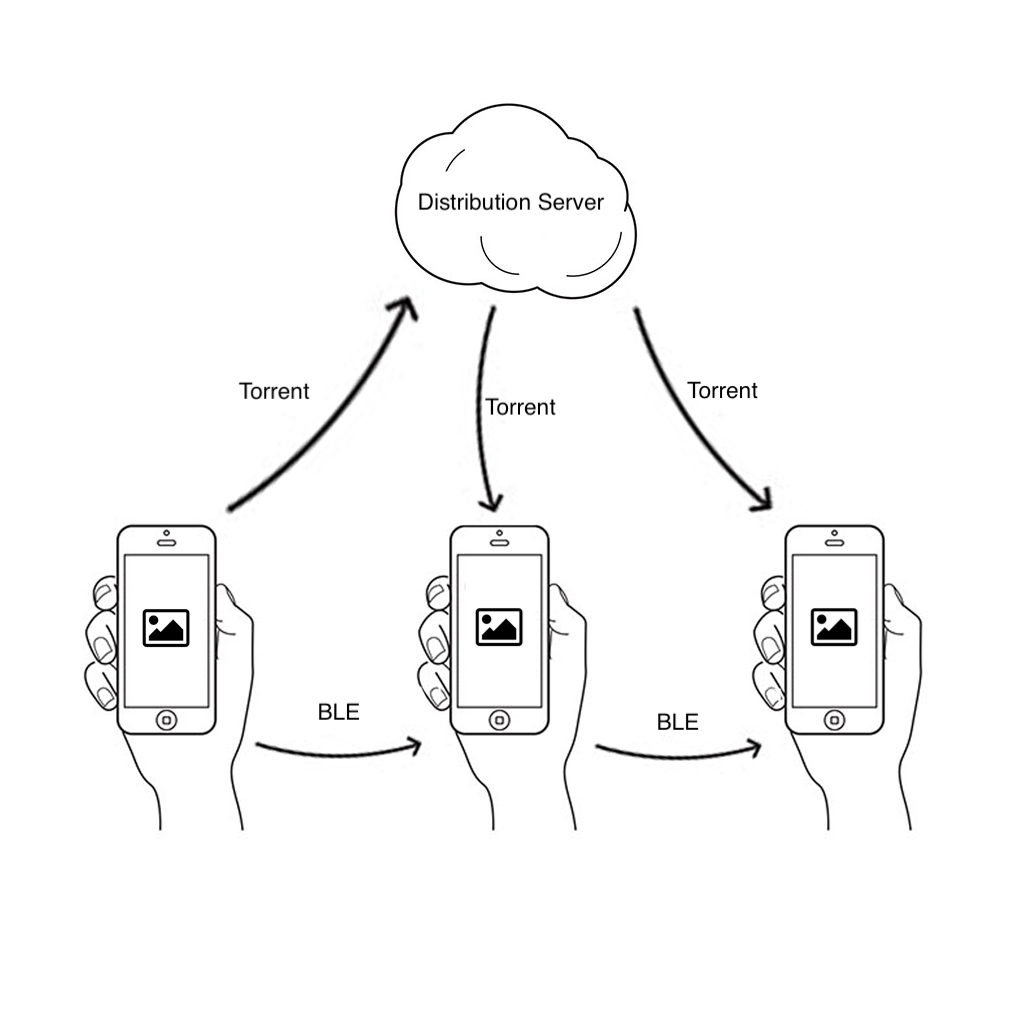
\includegraphics[width=\columnwidth]{overview.jpg}
    \lfig{system-overview}
    \vspace{-5mm} % use negative white space to fix too large gaps
	\caption{System Overview~\cite{estimote}}
\end{figure}

\section{Work Packages}
We figured out that working in the past group structures allowed developers to be flexible but also effective in their work. As such, we define broad tasks with specific goals.
In the following, we present tasks, that when done, result in a robust and well-working app.

\begin{itemize}
        \item {\bf WP1}:  Build an Android front-end that can take pictures and temporarily saves it in a local storage.    
        \item {\bf WP2}:  Build an Android back-end which acts as a node. 
        It should be able to transfer files from one device to another, and save it to the local storage.
        \item {\bf WP3}: Build the transition between WP1 and WP2 such that all transmitted files are displayed on the receiver using the front-end.    
        \item {\bf WP4}: Initialize and configure backend server which is supposed to serve as a tracker.    
        \item {\bf WP5}: Create all API endpoints which accept device ID's and picture-identifiers, and checks which photos are delivered to which devices. 
        The uuid can act as an unique identifier for each node.    
        \item {\bf WP6}: Implement P2P logic in the node backend that pings other phones for a photo, if a photo was not yet received (which is determined by the received photo id's). 
        \item {\bf WP7}: Extensive usage testing and debugging.
\end{itemize}
 
\section{Milestones}


\subsection{Schedule}
We form a temporal schedule on what tasks should be achieved, sorted by upcoming dates.
\begin{enumerate}
\item  \textbf{24. Nov. 2017}: We plan on finishing the work packages that are considered part of the app, namely \textit{WP1} and \textit{WP2}, .
\item  \textbf{1. Dec. 2017}: We intend to finish setting up the central tracker, and all it's API functions. These are part of \textit{WP3} and \textit{WP4}.
\item \textbf{8. Dec. 2017}: We plan to do a naive implementation of the entire system, where the tracker communicates with the phones the photos to be downloaded, and the photos are communicated between the individual nodes. This is concluded by \textit{WP5} and  \textit{WP6} 'putting the components together'.
\item \textbf{15. Dec. 2017}: Assuming all went as planned, we would try to test the network on a multi-node connection ($n < 3$), identifying bugs and generally debugging the system. 
We would possibly try to identify network congestion behaviour and try to optimize these (\textit{WP7}).
\end{enumerate}


\subsection{Assignment to team members}
Luckily, all tasks are extensive enough that a majority of team members can work on the individual working packages individually. 
As such, for each deadline (\textit{24. Nov. 2017}, \textit{1. Dec. 2017}, \textit{8. Dec. 2017}, \textit{15. Dec .2017}), we plan to split the team into two sub-sections, each of which handles one working package. Within each working package, we intend to have a flexible schedule amongst team-members, as this has proven to be effective in the past few Android projects. 
The last part (\textit{WP7}) is not well-predictable as of now. 
Our previous experience has shown us that collectively listing issues and working on these issues one-by-one has proven to be an effective way to debug and optimize our program.

\bibliographystyle{abbrv}
\bibliography{report}  % sigproc.bib is the name of the Bibliography in this case
% You must have a proper ".bib" file

%\balancecolumns % GM June 2007

\end{document}
